\chapter{Simulation corrections}
\label{chap:simulation-corrections}

%\chapterquote{}{}

\section{Introduction}

This chapter details the corrections applied to the Monte Carlo (MC) simulated events aimed at improving the description of observed events (data) by the MC.  These corrections are typically understood in terms of a scale multiplied to a quantity, also known as a scale-factor, hence a scale-factor of one represents no deviation from the nominal MC prediction. There are two main categories of corrections used in this analysis. The first corresponds to changing the weighting of a MC event, known as an event-based correction. The weight given to a MC event is the product of the cross-section of the particular process and the integrated luminosity, $\sigma \mathcal{L}$. The cross-section $\sigma$ is calculated to the highest order available in both the strong and electroweak coupling constants, whereas the luminosity $\mathcal{L}$ is measured by the \CMS and surrounding detectors. Event-based corrections will scale this weight on an event-by-event basis, however, the sum of the weights over all events should remain unchanged. The second set of corrections represents a shift in a parameter, such as altering the momentum of an object, hereby known as an object-based correction.

Typical aggregation of information is in the form of histograms where data in a particular bin is determined from the total number of events within the bin's criteria, whereas the MC contribution is a sum over the weights for the same criteria. Therefore, the event-based corrections simplify to a scale up or down to an event's contribution in the sum. However, object-based correction alter which bin the event may fall in. Both corrections, even if unity, are associated with an uncertainty to alter the correction up or down resulting in an alternative histogram under different variation hypotheses. These hypotheses are used later in the statistical interpretation of the results.

An event-based correction is determined by measuring the efficiency of a selection or requirement in data, \effdata, and again in MC, \effmc, parameterised in terms of observables $\vec{x}$ resulting in a scale-factor, $\hat{f}$, of
%
\begin{equation}
    \hat{f}(\vec{x}) = \frac{\effdata(\vec{x})}{\effmc(\vec{x})}\ .
\end{equation}
%
This reweighting procedure attempts to have MC replicate the observed efficiency for a particular selection. The efficiencies are measured with a few different techniques, discussed in detail below.


\subsection{Tag and probe method}

A common technique to measure the efficiency in data is known and the tag and probe method. This technique involves the selection of events containing two candidates: a tag which must pass a tight set of restrictions $T$ to firmly avoid misidentification, and a probe which passes very loose requirements $P$.  The events are such that the tag infers knowledge of the probe, for example, in \IDYll where one lepton is a tag and the other a probe. The efficiency of a selection $S$, given the probe requirements $P$, is determined by counting events:
%
\begin{equation}
    \varepsilon(S|P) = \frac{N(S\cap T\cap P)}{N(T\cap P)}\ ,
\end{equation}
%
where $N(R)$ is the number of events passing some set of requirements $R$. For a tag and probe from a \PZ boson decay the event counting is taken from the signal by performing a maximum likelihood fit to the \PZ peak with a falling background. A similar procedure can be performed in MC, however, knowledge of the generator-level objects and process omits the need for a tag. Other techniques in use are detailed in line.


\section{Trigger Efficiency}

The trigger selection discussed in Sec.~\ref{sec:baseline-selection} collect a particular set of events for the analysis; however, limitations in the reconstruction available to the \HWT and \SWT results in a loss of events. To replicate the data collection in simulated events the efficiency of a trigger selection is measured. The trigger selections are split into the muon, electron and \ptmiss categories.


\subsection{Muon trigger efficiency}

The muon trigger efficiency \cite{CMS-DP-2017-056} is measured with the tag and probe method where the tag selection $T$ and probe selection $P$ must pass the full set of analysis requirements apart from the \pt and $\eta$ criteria for the probe. This allows the parameterisation of the muon efficiency with \pt and $\eta$ as the trigger performance is expected to be highly dependent on these variables. The tag is also required to cause the event to pass the muon trigger selection such that the event is stored. The events are subsequently split into all probes and those passing the muon triggers with further division into independent \pt and $\eta$ bins. In each category, the maximum likelihood fit is performed to the invariant mass of the two muons to extract the signal and background contributions in each bin. The signal is modelled as a Breit-Wigner convoluted by a gaussian distribution and the background is modelled as a falling exponential.  The efficiency is determined in each bin from the ratio of signal events where the probe passes the muon trigger selection to signal events without this requirement. The statistical uncertainty on the signal events is propagated through to the efficiencies. Additional systematic uncertainties are determined by performing the fit varying, in turn, the number of invariant mass bins, invariant mass range, signal and background models, tag selection and probe multiplicity. During the 2016 data-taking period, saturation issues in the pre-amplifier chips for the tracker resulted in a loss of hits. This effect was mitigated in the later part of this period and further reduced by a re-processing of the data. Nevertheless, the muon trigger efficiencies are split into the initial part and final part of the data-taking period, as shown in Fig.~\ref{fig:muon-trigger-efficiency}.

\begin{figure}[htb]
    \centering
    \begin{subfigure}[b]{0.49\textwidth}
        \centering
        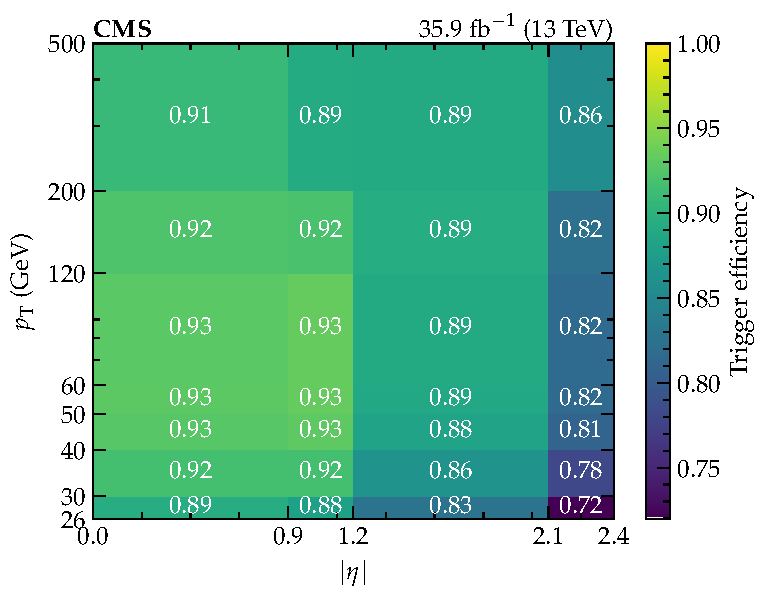
\includegraphics{chapters/041_corrections/images/efficiencies/triggers/muons/muon_RunBCDEF_trigger_efficiency.pdf}
        \caption{Initial data-taking period}
        \label{subfiga:muon-trigger-efficiency}
    \end{subfigure}
    \hfill
    \begin{subfigure}[b]{0.49\textwidth}
        \centering
        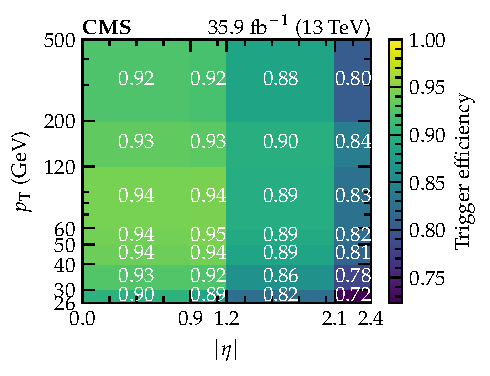
\includegraphics{chapters/041_corrections/images/efficiencies/triggers/muons/muon_RunGH_trigger_efficiency.pdf}
        \caption{Final data-taking period}
        \label{subfigb:muon-trigger-efficiency}
    \end{subfigure}
    \caption[Muon trigger efficiency measurements.]{
        Muon trigger efficiencies parameterised by its \pt and \aeta, split by the data-taking period. The trigger efficiency is lower in the endcaps where the muon background rate is larger and for low \pt muons where the track reconstruction is poorer. Inefficiencies for high \pt muons result from misidentified charged hadrons or issues in reconstructing the \pt for straight tracks. Most of the trigger efficiency arises from the \HWT decision which is heavily constrained by the timing budget. The differences between the data-taking periods are at most $2\%$, with significant overlap within the uncertainties.
    }
    \label{fig:muon-trigger-efficiency}
\end{figure}

This efficiency, $\varepsilon_i$, is associated to a single muon; however, events collected with higher muon multiplicities were triggered by any of the muons, hence the efficiency associated with the event, $\varepsilon$, for any number of muons is
%
\begin{equation}\label{eq:electron-event-trigger-efficiency}
    \varepsilon = 1 - \prod_{i\in\mathrm{muons}} ( 1 - \varepsilon_i )\ ,
\end{equation}
%
as follows from a binomial distribution where at least one muon must pass the trigger selection. This efficiency scales the MC event weight in regions collected by the muon triggers with a luminosity-weighted average of the initial and final data-taking periods.


\subsection{Electron trigger efficiency}

The electron trigger efficiency measurement \cite{CMS-DP-2017-004} follows a similar procedure to the muons. The analysis selection is applied to the tag and the probe, with relaxed kinematic criteria. The pair of electrons are formed into a \PZ boson candidate with a fit to the invariant mass distribution to extract the signal contribution and determine the efficiency of the electron trigger selection. Systematic uncertainties are determined with the same method detailed for the muon trigger efficiencies. The efficiencies for the electron trigger selection is shown in Fig.~\ref{fig:electron-trigger-efficiency} and follow the same event-based efficiency in Eq.~\ref{eq:electron-event-trigger-efficiency}.

\begin{figure}[htb]
    \centering
    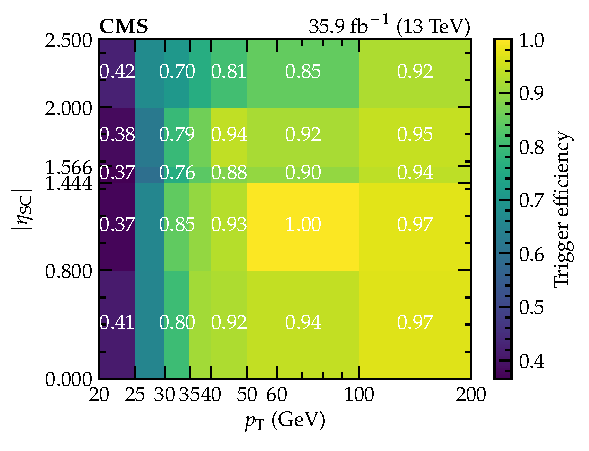
\includegraphics{chapters/041_corrections/images/efficiencies/triggers/electrons/electron_trigger_efficiency.pdf}
    \caption[Electron trigger efficiency.]{
        Electron trigger efficiency with a threshold of ${\pt>\SI{27}{GeV}}$, parameterised with the \pt and absolute supercluster position in $\eta$, $|\eta_{\mathrm{SC}}|$. The low \pt inefficiency is driven by the trigger threshold and the efficiency in the partially uninstrumented gap in the \ECAL is shown in the bin ${1.444<|\eta_{\mathrm{SC}}|<1.566}$.
    }
    \label{fig:electron-trigger-efficiency}
\end{figure}


\subsection{\ptmiss trigger efficiency}\label{sec:met-trigger-efficiency}

The \ptmiss trigger paths collect events for the \metplusjets, \muplusjets, \dimuplusjets, \tauplusjets and the equivalent QCD multijet enriched sidebands. To measure the efficiency in data, an independent set of events are collected using the single muon triggers which may pass or fail the \ptmiss trigger requirements. Furthermore, the \ptmiss triggers primarily place a selection on the recoil which ignores the muons, allowing events to populate the tail of the recoil distribution. No reference trigger is required in MC and the efficiency is extracted from the trigger emulation. The results for \IZvvj, \IWlvj and \IDYllj shown in Fig.~\ref{fig:ptmiss-trigger-eff-noisotrack}, alongside the measurements from data in the \muplusjets and \dimuplusjets regions.

\begin{figure}[htb]
    \centering
    \begin{subfigure}[b]{0.49\textwidth}
        \centering
        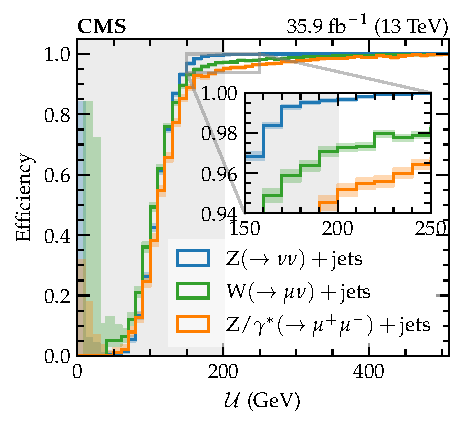
\includegraphics{chapters/041_corrections/images/efficiencies/triggers/met/met_trig_eff_mc_noisotrack.pdf}
        \caption{Simulation}
        \label{subfiga:ptmiss-trigger-eff-noisotrack}
    \end{subfigure}
    \hfill
    \begin{subfigure}[b]{0.49\textwidth}
        \centering
        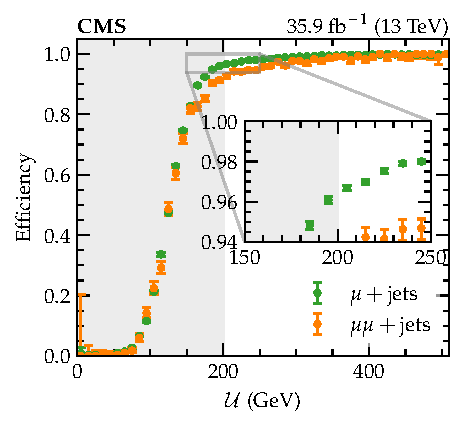
\includegraphics{chapters/041_corrections/images/efficiencies/triggers/met/met_trig_eff_data_noisotrack.pdf}
        \caption{Data}
        \label{subfigb:ptmiss-trigger-eff-noisotrack}
    \end{subfigure}
    \caption[Efficiency of the missing energy triggers in data and simulation.]{
        The dependence of the \ptmiss trigger efficiency on the offline recoil $\mathcal{U}$. The efficiency below $\SI{200}{GeV}$ (grey band) is shown, however, these event are removed in the final analysis. The uncertainty bands represent the $68.2\%$ asymmetric confidence interval on a binomial distribution for a given total number of event with a fraction passing the selection. This band only includes the statistical uncertainty in both simulation and data.
    }
    \label{fig:ptmiss-trigger-eff-noisotrack}
\end{figure}

The lower efficiency measured in data is a result of the evolution of trigger paths to higher thresholds as the beam luminosity increased throughout the 2016 data-taking period, whereas the simulated trigger efficiency is primarily controlled by the lowest threshold. The impact of the evolving trigger paths in data is replicated in MC by applying a scale factor correction determined from the ratio of data to MC efficiency, parameterised with the recoil.  However, a clear efficiency difference is observed between the various muon multiplicity regions. In fact, the \SWT muon collection is not perfectly aligned with the offline reconstructed collection causing some muons to be included in the \SWT recoil calculation leading to values below the thresholds. This is significantly mitigated by the addition of a \ptmiss trigger path which selects events with a \ptmiss above $\SI{75}{GeV}$ and an isolated track with ${\pt>\SI{50}{GeV}}$. This recovers events where the muon was misidentified at the \SWT level, however, still classified as an isolated track. The corresponding trigger efficiency measurements are shown in Fig.~\ref{fig:ptmiss-trigger-eff-isotrack}, with a significant improvement between the muon multiplicity regions.
%
\begin{figure}[htb]
    \centering
    \begin{subfigure}[b]{0.49\textwidth}
        \centering
        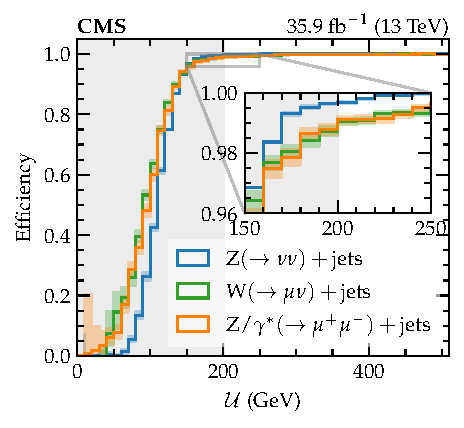
\includegraphics{chapters/041_corrections/images/efficiencies/triggers/met/met_trig_eff_mc.pdf}
        \caption{Simulation}
        \label{subfiga:ptmiss-trigger-eff-isotrack}
    \end{subfigure}
    \hfill
    \begin{subfigure}[b]{0.49\textwidth}
        \centering
        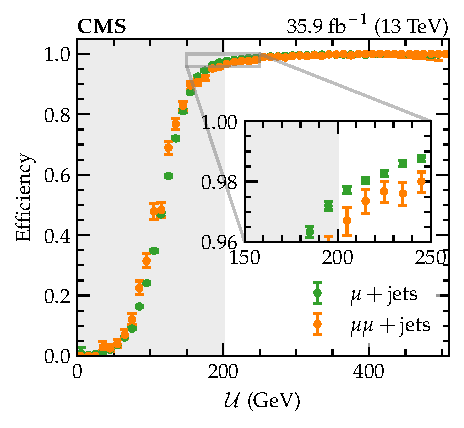
\includegraphics{chapters/041_corrections/images/efficiencies/triggers/met/met_trig_eff_data.pdf}
        \caption{Data}
        \label{subfigb:ptmiss-trigger-eff-isotrack}
    \end{subfigure}
    \caption[Missing energy trigger efficiency measurements with the isolated track selection.]{
        The \ptmiss trigger efficiency measurements similar to Fig.~\ref{fig:ptmiss-trigger-eff-noisotrack}, with the addition of the isolated track selection.
    }
    \label{fig:ptmiss-trigger-eff-isotrack}
\end{figure}

The \ptmiss trigger scale factors are taken from the \muplusjets region where the statistical uncertainty is the lowest. The remaining difference in the scale factors between the \muplusjets and \dimuplusjets regions is taken as a systematic uncertainty to cover residual effects from the muon mismatch between the \SWT and offline. The effect of using the muon triggers as a reference in data is emulated in simulation and the difference between the nominal scale factor is taken as a systematic uncertainty. A final systematic uncertainty is determined by the difference in the scale factors in an independent region, namely the \muplusjets QCD enriched sideband. The scale factors and the associated systematic uncertainties are shown in Fig.~\ref{fig:ptmiss-trigger-sf}.
%
\begin{figure}[htb]
    \centering
    \begin{subfigure}[b]{0.45\textwidth}
        \centering
        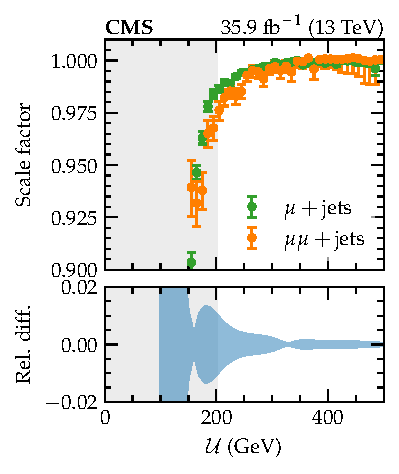
\includegraphics{chapters/041_corrections/images/efficiencies/triggers/met/met_trig_sf_muonsyst.pdf}
        \caption{Muon multiplicity}
        \label{subfiga:ptmiss-trigger-sf}
    \end{subfigure}
    \hfill
    \begin{subfigure}[b]{0.45\textwidth}
        \centering
        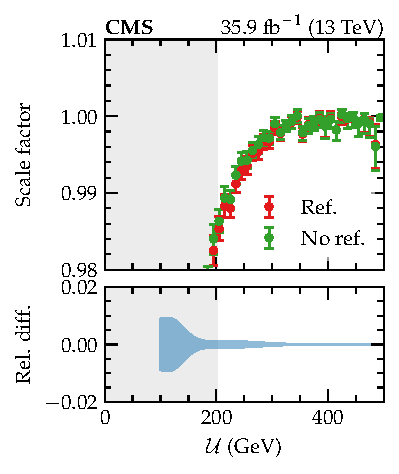
\includegraphics{chapters/041_corrections/images/efficiencies/triggers/met/met_trig_sf_refsyst.pdf}
        \caption{Reference trigger}
        \label{subfigb:ptmiss-trigger-sf}
    \end{subfigure}
    \\
    \begin{subfigure}[b]{0.45\textwidth}
        \centering
        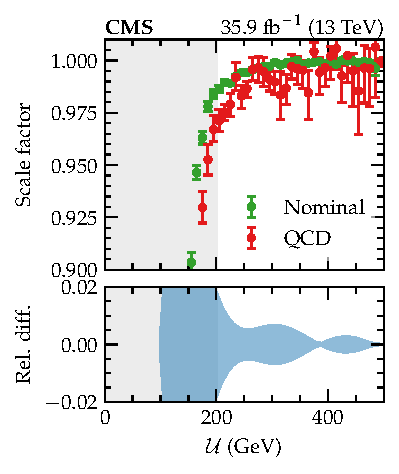
\includegraphics{chapters/041_corrections/images/efficiencies/triggers/met/met_trig_sf_qcdsyst.pdf}
        \caption{Independent sample}
        \label{subfigc:ptmiss-trigger-sf}
    \end{subfigure}
    \caption[Systematic uncertainties associated with the missing energy trigger efficiency measurements.]{
        The \ptmiss trigger scale factors measured for various regions to determine the central correction and relative difference between them for systematic uncertainties. The statistical uncertainties in the scale factors would artificially inflate the scale factors due to correlations between the bins, therefore, it is not used any further in the analysis.
    }
    \label{fig:ptmiss-trigger-sf}
\end{figure}
%
The reference trigger introduces a small bias of less than $0.5\%$, whereas the muon multiplicity systematic covers a $1\%$ effect and the QCD sideband a $2\%$ effect at ${\mathcal{U}=\SI{200}{GeV}}$ and drops off to a negligible level above $\SI{500}{GeV}$ where the efficiencies and scale factors plateau at $1$. The scale factors associated with the \muplusjets region in Fig.~\ref{subfiga:ptmiss-trigger-sf} is applied to all events collected by \ptmiss triggers to primarily correct for the changing conditions during data taking by up to $2\%$, with three systematic uncertainties propagated as alternative templates for the final statistical analysis to cover biases in the scale factor measurement.

The muon multiplicity systematic is decorrelated between the \metplusjets, \muplusjets and \dimuplusjets, allowing the systematic effect to pull each in separate directions. The reference trigger systematic is correlated among all regions. Similarly to the muon multiplicity, the independent sample systematic is decorrelated among all regions. This correlation scheme is a conservative estimate of the underlying uncertainty with the estimation of the \ptmiss trigger scale factors.

\section{Object-based corrections}

Corrections based on the physics objects of an event may alter the weight of the event and will be discussed here, along with corrections to particle kinematics. Furthermore, the selection discussed in Sec.~\ref{sec:categorisation} are not strict requirements on MC events. In particular, events with an object and an associated scale-factor $f$ will contribute to the object selection regions by a weight $f$. However, this event will also contribute to object veto regions by a weight $1-f$ such that the total contribution of the event across all regions becomes $1$, leaving the overall cross-section unchanged. When $f=1$ the strict veto requirements are recovered and the event does not enter the object vetoing regions. The uncertainty on the efficiency of a selection is encoded in the scale-factor, $\delta f$, such that the weight where the event is vetoed is
%
\begin{equation}
    1 - f = 1 - \mathcal{N}_f(f_0,\delta f_1) = 1 - (f_0 + \mathcal{N}_f(0,1)\delta f_1)\ ,
\end{equation}
%
where $f_0$ is the central value of the scale-factor, $\delta f_1$ is its $1\sigma$ variation and $\mathcal{N}_f(\mu,\sigma)$ is a gaussian distributed random variable with a mean $\mu$ and width $\sigma$. Therefore, MC events vetoed may still contribute to a region, albeit weighted down or possibly negatively. Such a procedure is performed with muons, electrons, photons, \Ptauh-leptons and $b$-tagged jets for both the veto and selection definitions.


\subsection{Muons}

Muons are formed from tracks with identification and isolation requirements to reduce misidentification. The efficiency in selecting muons is factorised into
%
\begin{equation}
    \varepsilon_{\mu} = \varepsilon_{\mu}(\mathrm{ID}|\mathrm{track}) \varepsilon_{\mu}(\mathrm{Iso}|\mathrm{ID})\ ,
\end{equation}
%
where the track collection efficiency is near $100\%$ and hence omitted. The parameter $\varepsilon(\mathrm{ID}|\mathrm{track})$ is the identification efficiency for a given set of tracks and $\varepsilon(\mathrm{Iso}|\mathrm{ID})$ is the isolation efficiency given a collection of muons passing identification requirements. Since the analysis uses two muon identification and isolation requirements the efficiency must be measured for both the veto and selection criteria. The measurement is performed using the tag and probe technique with the tag passing a tight set of requirements to ensure minimal misidentifications and the probe defined as a set of tracks or muons with an isolation requirement \cite{CMS-DP-2017-007}. Similarly to the muon trigger efficiency measurements, the events are split into bins of lepton \pt and $\eta$. A likelihood fit to the invariant mass distribution of each bin is independently performed to extract the signal contribution for the numerator and denominator of the efficiency: probes passing the isolation and identification requirements and all probes, respectively. A similar approach is performed in MC, however, the distinction of signal events is known, bypassing the need for a fit allowing for the simple counting of events.

During the 2016 data-taking period, saturation issues in the pre-amplifier chips for the tracker resulted in a loss of hits. This effect was mitigated in the later part of this period and further reduced by a re-processing of the data. Nevertheless, the identification and isolation efficiencies are split into the initial part and final part of the data-taking period. The ratio of the efficiencies measured in data and MC for each period is shown in Fig.~\ref{fig:muon-id-scale-factors} and \ref{fig:muon-iso-scale-factors} and subsequently the product of the identification and isolation scale-factors is applied as a correction to MC.

\begin{figure}[htb]
    \centering
    \begin{subfigure}[b]{0.49\textwidth}
        \centering
        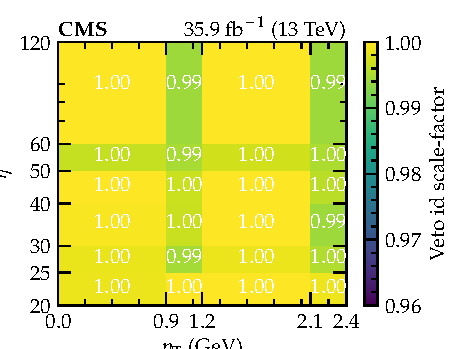
\includegraphics{chapters/041_corrections/images/efficiencies/objects/muons/muon_id_loose_runbf.pdf}
        \caption{Initial data-taking period}
        \label{subfiga:muon-id-scale-factors}
    \end{subfigure}
    \hfill
    \begin{subfigure}[b]{0.49\textwidth}
        \centering
        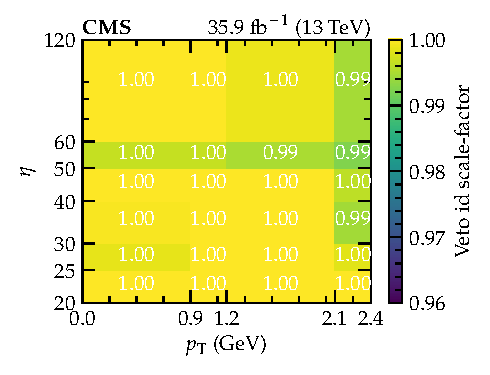
\includegraphics{chapters/041_corrections/images/efficiencies/objects/muons/muon_id_loose_rungh.pdf}
        \caption{Final data-taking period}
        \label{subfigb:muon-id-scale-factors}
    \end{subfigure}
    \\
    \begin{subfigure}[b]{0.49\textwidth}
        \centering
        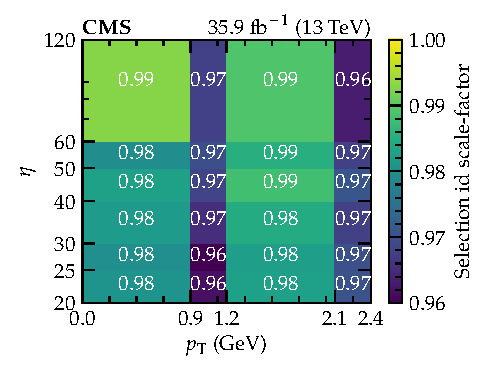
\includegraphics{chapters/041_corrections/images/efficiencies/objects/muons/muon_id_tight_runbf.pdf}
        \caption{Initial data-taking period}
        \label{subfigc:muon-id-scale-factors}
    \end{subfigure}
    \hfill
    \begin{subfigure}[b]{0.49\textwidth}
        \centering
        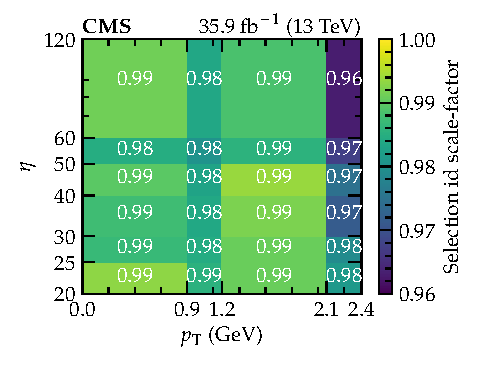
\includegraphics{chapters/041_corrections/images/efficiencies/objects/muons/muon_id_tight_rungh.pdf}
        \caption{Final data-taking period}
        \label{subfigd:muon-id-scale-factors}
    \end{subfigure}
    \caption[Corrections to simulated muon identification efficiencies.]{
        Muon identification (id) scale corrections applied to MC, parameterised with the muon \pt and \aeta. The top row shows the scale-factors for veto muons with corrections less than $1\%$ as a result of the basic selection. The bottom row shows the scale-factors for selection muons with corrections from {$1$--$4\%$} with the largest discrepancies on the edges of the endcaps (${0.9<\aeta<1.2}$ and ${2.1<\aeta<2.4}$) where the muon identification modelling does not perform as well in MC. 
    }
    \label{fig:muon-id-scale-factors}
\end{figure}

\begin{figure}[htb]
    \centering
    \begin{subfigure}[b]{0.49\textwidth}
        \centering
        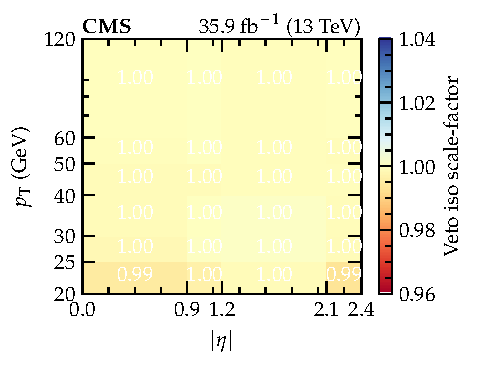
\includegraphics{chapters/041_corrections/images/efficiencies/objects/muons/muon_iso_loose_runbf.pdf}
        \caption{Initial data-taking period}
        \label{subfiga:muon-iso-scale-factors}
    \end{subfigure}
    \hfill
    \begin{subfigure}[b]{0.49\textwidth}
        \centering
        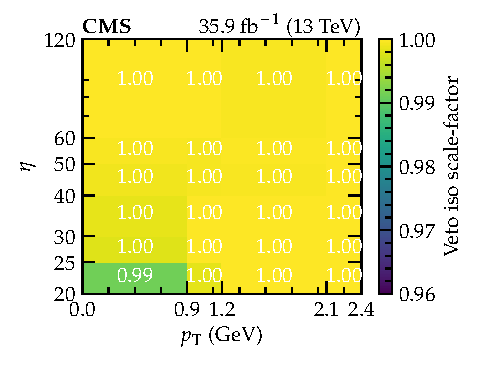
\includegraphics{chapters/041_corrections/images/efficiencies/objects/muons/muon_iso_loose_rungh.pdf}
        \caption{Final data-taking period}
        \label{subfigb:muon-iso-scale-factors}
    \end{subfigure}
    \\
    \begin{subfigure}[b]{0.49\textwidth}
        \centering
        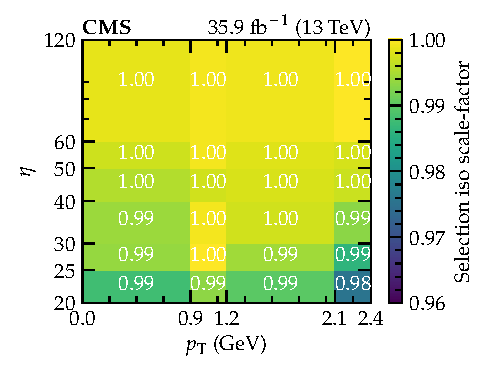
\includegraphics{chapters/041_corrections/images/efficiencies/objects/muons/muon_iso_tight_runbf.pdf}
        \caption{Initial data-taking period}
        \label{subfigc:muon-iso-scale-factors}
    \end{subfigure}
    \hfill
    \begin{subfigure}[b]{0.49\textwidth}
        \centering
        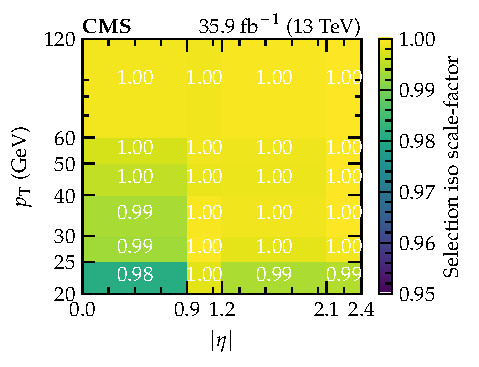
\includegraphics{chapters/041_corrections/images/efficiencies/objects/muons/muon_iso_tight_rungh.pdf}
        \caption{Final data-taking period}
        \label{subfigd:muon-iso-scale-factors}
    \end{subfigure}
    \caption[Corrections to simulated muon isolation efficiencies.]{
        Muon isolation (iso) scale corrections applied to MC, parameterised with the muon \pt and \aeta. The modelling of the isolation in MC is better than the identification with at most $2\%$ difference for selection muons with discrepancies only in the low \pt region. The $z$-axis range is the same as the muon identification scale factor in Fig.~\ref{fig:muon-id-scale-factors}.
    }
    \label{fig:muon-iso-scale-factors}
\end{figure}


\subsection{Electrons and Photons}

The efficiency of the identification and isolation of electromagnetic showers are measured with the tag and probe technique in a similar manner to the muon-based efficiencies \cite{CMS-DP-2017-004}. A fit to the invariant mass distribution of electron pairs is performed to extract the signal yield in various probe \pt and $\eta$ bins. This allows the efficiencies to be determined with analogous measurements in MC with the counting method.  Systematic uncertainties are determined from the variation in efficiencies from altering the tag selection, signal model (template from MC or fully parametric), background model, MC generator (LO against NLO), and additional sources for the photon identification efficiency to account for differences in the electron and photon showers. The ratio of the efficiency in data and MC is determined, shown in Fig.~\ref{fig:egamma-id-iso-efficiency} and applied as a correction to MC.

\begin{figure}[htb]
    \centering
    \begin{subfigure}[b]{0.49\textwidth}
        \centering
        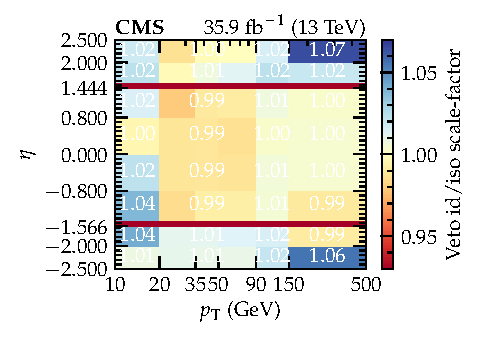
\includegraphics{chapters/041_corrections/images/efficiencies/objects/electrons/electron_idiso_veto_sf.pdf}
        \caption{Electron veto}
        \label{subfiga:egamma-id-iso-efficiency}
    \end{subfigure}
    \hfill
    \begin{subfigure}[b]{0.49\textwidth}
        \centering
        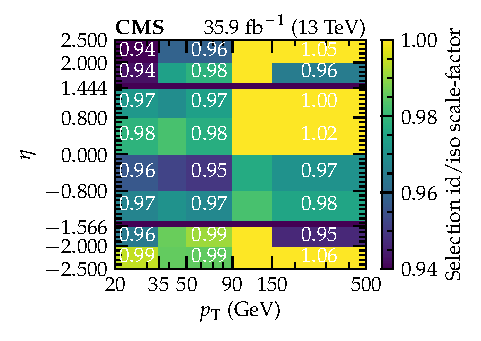
\includegraphics{chapters/041_corrections/images/efficiencies/objects/electrons/electron_idiso_tight_sf.pdf}
        \caption{Electron selection}
        \label{subfigb:egamma-id-iso-efficiency}
    \end{subfigure}
    \\
    \begin{subfigure}[b]{0.49\textwidth}
        \centering
        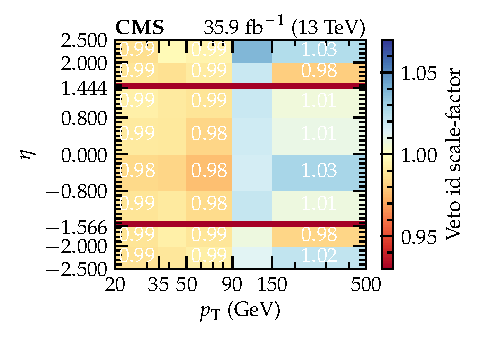
\includegraphics{chapters/041_corrections/images/efficiencies/objects/photons/photon_id_veto_sf.pdf}
        \caption{Photon veto}
        \label{subfigc:egamma-id-iso-efficiency}
    \end{subfigure}
%    \hfill
%    \begin{subfigure}[b]{0.49\textwidth}
%        \centering
%        \includegraphics{}
%        \caption{Caption}
%        \label{subfigd:egamma-id-iso-efficiency}
%    \end{subfigure}
    \caption[Corrections to simulated electron and photon identification efficiencies.]{
        Electron and photon identification scale-factors for the various analysis-level object categorisations. The bands at ${1.444<\aeta<1.566}$ correspond to the partially uninstrumented gap in the \ECAL. The corrections typically arise from the mismodelling of the interactions of electromagnetic particles with the inner detector material resulting in photon conversions and Bremsstrahlung, particularly in the endcaps. 
    }
    \label{fig:egamma-id-iso-efficiency}
\end{figure}

In addition, the efficiency for the reconstruction of GSF tracks matched to \ECAL deposits is measured with the same method and shown in Fig.~\ref{fig:electron-reco-efficiency}. Similarly, the efficiency from vetoing photons with consistent track in the pixel detector is measured with a similar method in \IDYmmg, where the tag consists of a muon pair and the probe a final state radiated photon. The ratio of the efficiency in data and MC for the GSF track veto is shown in Fig.~\ref{fig:photon-trackveto-efficiency}.

\begin{figure}[htb]
    \centering
    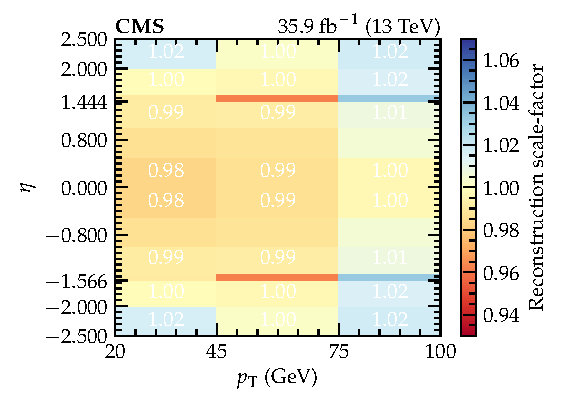
\includegraphics{chapters/041_corrections/images/efficiencies/objects/electrons/electron_reco_sf.pdf}
    \caption[Corrections to simulated electron reconstruction efficiency.]{
        Electron scale-factors associated with the reconstruction of electrons from tracks and \ECAL deposits. The \ECAL partially uninstrumented gap at ${1.444<\aeta<1.566}$. Mostly a good agreement between data and MC with deviations for low \pt and endcap electrons, again affected by material interactions.
    }
    \label{fig:electron-reco-efficiency}
\end{figure}

\begin{figure}[htb]
    \centering
    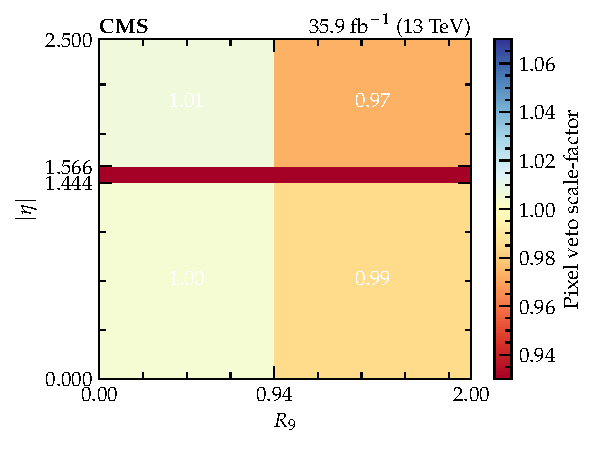
\includegraphics{chapters/041_corrections/images/efficiencies/objects/photons/photon_pixelveto_sf.pdf}
    \caption[Corrections to photon pixel veto efficiency.]{
        Photon pixel veto scale-factors parameterised by \aeta and $R_9$, the ratio of energy deposited in a $3\times 3$ grid of crystals surrounding the seeding crystal with the full supercrystal energy. The $R_9$ variable is sensitive to unconverted ($R_9\lesssim 0.94$) and converted ($R_9\gtrsim 0.94$) photons. The pixel veto removes photon candidates matched to tracks in the pixel detector.
    }
    \label{fig:photon-trackveto-efficiency}
\end{figure}

Finally, the difference in the scale and resolution of electrons and photons in data and MC is measured from the impact on the mean and width of. Therefore, an additional correction is determined by probing the $\eta$-dependent corrections with a selection to enhance the effect of this correlation. Along with these corrections are associated systematic uncertainties to cover the modelling in MC from an alternative event generator, statistical uncertainties in the data due to trigger prescales, dependence of the corrections over the data taking period, constituent particle energy uncertainties, and the residual difference between the dijet, \Igj and \IDYllj samples after all corrections have been applied.

In addition to the jet energy response difference between data and MC the resolution is corrected for by comparing the balance of jets in a dijet event.  The scale determined to correct the MC resolution of the dijet balance is applied to MC jets by smearing their energies with a random variable sampled from a gaussian distribution with a scaled width. Systematic uncertainties are determined by comparing the results to the particle-level imbalance, the effect of removing particles below $\SI{10}{GeV}$, non-gaussian tails in the resolution due to rare detector effects and the \pt-dependence is propagated through the smearing.

All these corrections, and uncertainties, are propagated through all jet-related quantities such as the missing transverse momentum where the jet energy correction $k_i$, encoding both scale and resolution corrections, results in a shift in the \ptmiss according to
%
\begin{equation}\label{eq:ptmiss-type1-corr}
    \vecptmiss \mapsto \vecptmiss + \sum_{i\in\mathrm{jets}}\vec{p}_{\mathrm{T},i} \left( 1 - k_i \right)\ ,
\end{equation}
%
where the sum is over clustered jets, i.e. ${\pt>\SI{15}{GeV}}$. The corrected \ptmiss quantity is used in subsequent derivatives such as the recoil.


\subsubsection{\Ptauh-tagged jets}

The jet energy corrections discussed above are determined under the assumption that the jet originates from a parton. Therefore, the corrections are not applied to \Ptauh-tagged jets, instead a scale-factor is determined to correct the efficiency of \Ptauh-lepton identification in MC. The efficiency in data is measured using the tag and probe method in \IDYtt decays, where one $\tau$-lepton decays into a well reconstructed muon to tag the event and the other into one of the hadronic decay modes to probe the identification. A fit is performed to the invariant mass of the visible particles to extract the signal contribution with templates taken from MC for the signal and most backgrounds. Systematic uncertainties on the identification efficiency are determined from the background normalisation, \ptmiss uncertainties and limited sample sizes \cite{Sirunyan:2018pgf}. The scale-factors and uncertainties to correct the \Ptauh identification efficiency in MC is shown in Fig.~\ref{fig:tau-id-scale-factors}.

\begin{figure}[htb]
    \centering
    \begin{subfigure}[b]{0.49\textwidth}
        \centering
        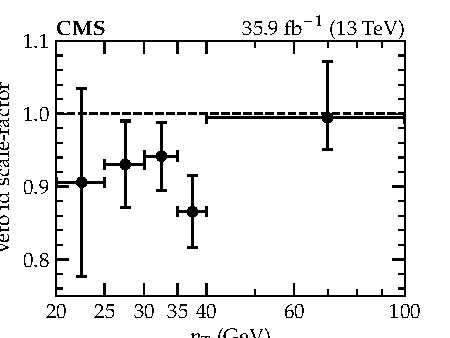
\includegraphics{chapters/041_corrections/images/efficiencies/objects/taus/tau_id_veto_sf.pdf}
        \caption{Veto identification}
        \label{subfiga:tau-id-scale-factors}
    \end{subfigure}
    \begin{subfigure}[b]{0.49\textwidth}
        \centering
        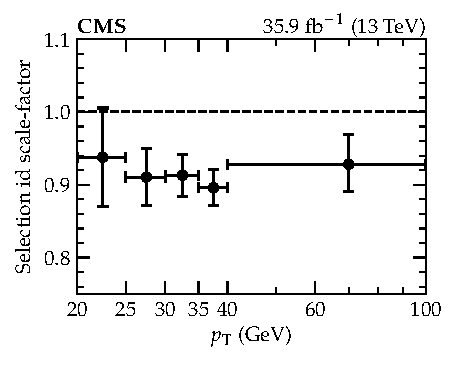
\includegraphics{chapters/041_corrections/images/efficiencies/objects/taus/tau_id_tight_sf.pdf}
        \caption{Selection identification}
        \label{subfigb:tau-id-scale-factors}
    \end{subfigure}
    \caption[Corrections to $\tau$-tagged jet efficiency.]{
        \Ptauh identification scale-factors parameterised by the \Ptauh \pt. The dashed line is placed at a scale-factor of $1$. The veto category is mostly consistent with $1$ while the selection category deviates by {$5$--$10\%$} as a result of attempting to reduce misidentifications by probing the complex structure of multiple hadronic $\tau$-lepton decays.
    }
    \label{fig:tau-id-scale-factors}
\end{figure}


\subsubsection{$b$-tagged jets}

Jets tagged as originating from $b$-hadrons have the jet energy corrections applied, however, the $b$-tagging discriminant is not perfectly modelled in MC due to detector simulation limitations and the accuracy of the generator modelling the parton shower and hadronisation. Therefore, a scale-factor is determined for the efficiency of $b$-tagging jets from QCD multijet, muon-enriched jet, dilepton \Itt and single lepton \Itt samples \cite{Sirunyan:2017ezt}. The efficiency is parameterised by the jet flavour (grouped in $b$, $c$ and $udsg$ flavours), \pt and $\eta$. In simulation, the tagging efficiency is calculated by matching jets to generated jets with a particular hadron flavour. Meanwhile, the data efficiency is measured with a pure sample with jets of a certain hadron flavour using a selection which does not bias the jets with respect to the variables in the tagging algorithm.  Systematic uncertainties associated to the $b$-tag scale-factors are determined by varying background normalisations, branching fractions of hadronic decays within the PDG uncertainties, reweighting the distribution of the number of tracks, jet energy scale uncertainties, electron and muon efficiencies and theoretical uncertainties from the event generators. The scale-factors associated with the $i$-enumerated $b$-tagged jet, $f_i$, is measured with a parameteric form with the \pt of the jet given by
%
\begin{equation}
    f_i(\pt) =
    \begin{cases}
        p_0 \left(1 + p_1 \pt\right)/\left(1 + p_2 \pt\right), & \text{$c$ and $b$-hadrons}\\
        p_0 + p_1 \pt + p_2 \pt^2 + p_3 \pt^3, & \text{$udsg$-hadrons}
    \end{cases}
\end{equation}
%
where $p_0$, $p_1$, $p_2$ and $p_3$ are parameters measured from a fit to the scale-factors in categories based on the jet flavour, \pt and $\eta$. In the context of this analysis, $b$-tagged jets are vetoed, therefore the event weight becomes
%
\begin{equation}
    w \mapsto w \prod_{i\in\mathrm{b-jets}} (1 - f_i)\ .
\end{equation}


\section{Luminosity}

The integrated luminosity $\mathcal{L}$ measured for the data-taking period directly scales the weight of a MC event. At \CMS the pixels, drift tubes, HF and other detectors perform complimentary measurements of the luminosity by rate counting, $R$, for visible processes with a cross-section $\sigma_{\mathrm{vis}}$. The luminosity is determined as
%
\begin{equation}
    \mathcal{L} = \frac{R}{\sigma_{\mathrm{vis}}}\ ,
\end{equation}
%
where the visible cross-section and calibrations of each detector is performed by conducting Van der Meer scans \cite{vanderMeer:296752} prior to data-taking collisions. The data collected during 2016 corresponds to an integrated luminosity of ${\SI{35.9}{fb^{-1}}}$ with uncertainties from the precision of the visible cross-section and calibration measurements along with extrapolations to data-taking collisions resulting in a $2.5\%$ uncertainty \cite{CMS:2017sdi} on the luminosity measurement.


\section{Pileup reweighting}

The pileup overlay applied to each simulated event is generated by the \PYTHIA package with the number of pileup vertices sampled from a poisson distribution with a tail to higher vertex multiplicities. In data, for a given instantaneous luminosity, the number of pileup vertices is expected to be poisson distributed. Therefore, a reweighting procedure corrects the MC distribution to reflect that observed in data, without altering the normalisation determined from the product of the process cross-section and the integrated luminosity. The number of interactions in data is estimated from the measured luminosity in each bunch crossing and the average total inelastic cross-section. Furthermore, data measurements are averaged over periods of constant instantaneous luminosity to compare with the mean of poisson distribution sampled in MC, rather than the number of vertices in a particular event. The total inelastic cross-section, measured by \CMS, is ${\SI{69.2}{mb}}$, with an uncertainty of $4.6\%$ represented by the bands in Fig.~\ref{fig:pu-reweighting}. These $\pm 1\sigma$ variations are propagated through to the \PZ invisible width measurement.

\begin{figure}[htb]
    \centering
    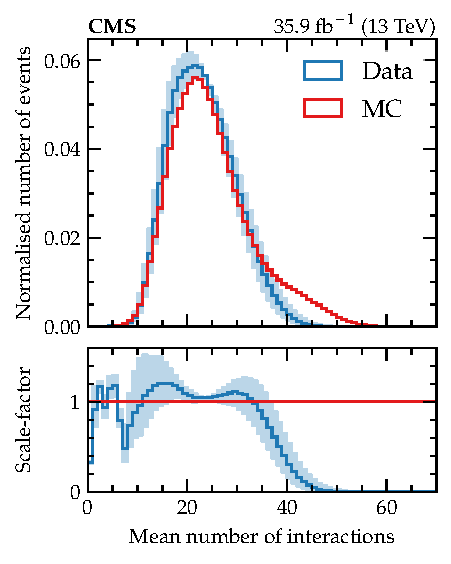
\includegraphics{chapters/041_corrections/images/pileup/pileup.pdf}
    \caption[Pileup distribution in data and simulation for reweighting.]{
         The distribution of the mean number of interactions the events are sampled from, closely following a poisson distribution with a long tail in MC. The uncertainty band is determined by varying the total inelastic cross-section by $4.6\%$. The average of the mean number of interactions in data is $22.7$, under the \LHC beam conditions provided during 2016.
    }
    \label{fig:pu-reweighting}
\end{figure}


\section{\ECAL timing degradation}

A gradual degradation in the \ECAL timing has caused some \HWT \ECAL towers to be associated with the incorrect bunch crossing (BX). The \HWT logic prevents three successive bunch crossings to be accepted to avoid buffer overflows.  Therefore, the deposit in the \ECAL is wrongly associated to an early crossing which may lead to a \HWT accept, later discarded in the \SWT where the timing issue is not present. However, the correct crossing is vetoed by the \HWT logic resulting in a loss in efficiency in the data collection. This primarily affects events with \ECAL deposits in the endcaps where the timing degradation is most prevalent.

The efficiency of this issue is measured by collecting immune events which occur three bunch crossings after a \HWT accepted crossing. The immune event is labelled as $\mathrm{BX}+0$ and the $n$-enumerated crossing before as $\mathrm{BX}-n$ and after as $\mathrm{BX}+n$. Since $\mathrm{BX}-3$ is accepted by the \HWT the crossings $\mathrm{BX}-2$ and $\mathrm{BX}-1$ are vetoed, hence they cannot veto $\mathrm{BX}+0$. Although these events are immune to the issue, they are tagged as events that would have been vetoed if $\mathrm{BX}-1$ or $\mathrm{BX}-2$ contains a \HWT object from $\mathrm{BX}+0$. However, the event is recovered since it is protected by the preceding $\mathrm{BX}-3$. The efficiency is determined from the set of immune events, with and without a problematic \HWT object. It is parameterised by the \pt and $\eta$ of the reconstructed jet associated with the problematic \HWT object. In MC the efficiency of this issue is determined from a product over the measured efficiencies associated to each object which is applied as a correction to the event weight. Along with this, a systematic uncertainty is determined from the statistical uncertainty of the immune sample or a conservative $20\%$ on the correction relative to $1$, whichever is largest.


\section{Theory corrections}\label{sec:theory-corrections}

The cross-section applied directly to the event weight of a MC process is calculated by theoretical predictions of the highest available order in the strong and electroweak (EW) coupling constants. Associated systematic uncertainties are determined by varying the QCD factorisation and renormalisation scale up and down by a factor of two. This is done for the independent variation of the two scales and the fully correlated variation, with the largest of the six variations taken as the systematic uncertainty. In addition, the uncertainties from the measurements of the sampled \NNPDF parton distribution functions (PDF) \cite{Ball:2014uwa} are propagated by 100 variations, each randomly sampled from the original distributions of the PDFs.

An alternative method is applied to the signal and dominant \IVj processes.  These are generated at NLO in the strong coupling constant, however, instead of scaling the normalisation up to the highest order available, a reweighting of the boson \pt distribution is performed for a more accurate prediction.  This approach reweights the MC to NNLO QCD and NLO EW with next-to-leading logarithm (NLL) EW corrections \cite{Lindert:2017olm}. This procedure scales the cross-section parameterised by the boson \pt, determined from the generated decay products (with photons within ${\Delta R<0.1}$ of charged leptons summed into their 4-momentum). Systematic uncertainties determined for the QCD corrections include variations in the factorisation and renormalisation scales with the addition of a possible boson \pt dependence and encoding the correlation between the \IZj and \IWj processes.

Another set of systematic uncertainties are determined for the EW corrections to cover higher-order effects and an additional systematic uncertainty on unaccounted contributions from diagrams of mixed order in the strong and EW coupling constants by taking the difference between an additive and factorised combination of the separate QCD and EW corrections. The PDF uncertainties are propagated with the same procedure as for other generated processes. The full set of uncertainties are detailed in Tab.~\ref{tab:qcdew-systematics}.

\begin{table}[htb]
    \centering
    \begin{tabular}{lccp{9cm}}
        \hline \hline
        Label & \IVj & Other & Description \\
        \hline
        \uncqcdone & \checkmark & \checkmark & Factorisation and renormalisation scale variations. \\
        \uncqcdtwo & \checkmark & & Boson \pt dependence of the QCD scales. \\
        \uncqcdthr & \checkmark & & Correlations between QCD effects in \IZj and \IWj processes. \\
        \hline
        \uncewone & \checkmark & & Unknown Sudakov logarithms beyond NNLO. \\
        \uncewtwo & \checkmark & & $5\%$ of the absolute full NLO EW correction for a conservative estimate of non-Sudakov factors. \\
        \uncewthr & \checkmark & & Difference between a naive and rigorous NLL Sudakov approximation. \\
        \hline
        \uncqcdewmix & \checkmark & & Mixing terms with strong and EW coupling vertices. \\
        \hline
        \uncpdf & \checkmark & \checkmark & 100 PDF variations. \\
        \hline \hline
    \end{tabular}
    \caption[Summary of the uncertainties associated to theoretical predictions.]{
        All systematic uncertainties included from the theory prediction of process cross-sections with a tick for which processes the uncertainty affects split into either \IVj or other processes. A brief description of each is given.
    }
    \label{tab:qcdew-systematics}
\end{table}


\section{\ptmiss calibration}\label{sec:ptmiss-calib}

The missing energy appears in the analysis selection as the recoil variable $\mathcal{U}$, with the criteria ${\recoil>\SI{200}{GeV}}$ driven by the trigger thresholds. This parameter acts as a proxy for the boson \pt in \IVj processes. The simulation modelling of the recoil as a proxy for the boson \pt is confirmed in data by calibration with \diellplusjets events. These events have an independent measure of the boson \pt through the dilepton \pt. Discrepancies in the modelling are typically due to the nonlinear response of the calorimeters to hadronic particles and the modelling of interactions with the inner detector. A schematic diagram of the event kinematics is shown in Fig.~\ref{fig:recoil-calib-diagram}.

\begin{figure}[htb]
    \centering
    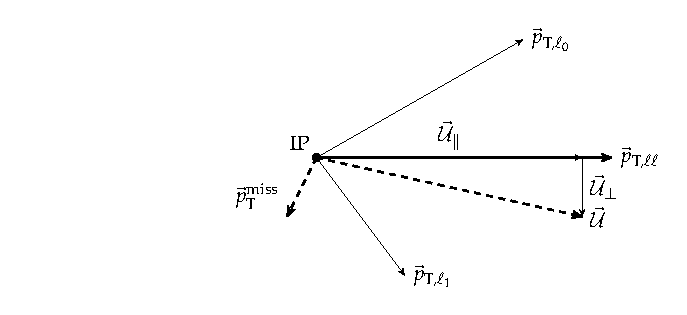
\includegraphics{diagrams/tikz/recoil_calib/recoil_calib.pdf}
    \caption[Kinematics diagram of a \IDYllj events.]{
        The $x$-$y$ plane kinematics of a \IDYllj event showing the momenta of the leading lepton $\ell_0$, subleading lepton $\ell_1$, their sum \vecptll; the missing transverse momentum \vecptmiss; the recoil, defined as $\vecrecoil=\vecptll+\vecptmiss$; and the parallel and perpendicular components of the recoil along the \vecptll axis, \vecrecoilpara and \vecrecoilperp respectively. The interaction point (IP) is at the centre. The missing energy is spurious as a result of mismeasurement, particles out of acceptance or from pileup vertices, and noise.
    }
    \label{fig:recoil-calib-diagram}
\end{figure}

The parallel component \vecrecoilpara probes imperfect calibrations of the \ptmiss typically from mismeasurement in the hadronic system, whereas the perpendicular component \vecrecoilperp probes the isotropic nature of the energy fluctuations from noise and pileup particles. The magnitude of the \vecrecoilpara subtracted by \vecptll along with the magnitude of the \vecrecoilperp are expected to be centred on the scale of the \ptmiss and a width corresponding to its resolution. The distribution of these variables is shown in Fig.~\ref{fig:recoil-calib-dists}.

\begin{figure}[htb]
    \centering
    \begin{subfigure}[b]{0.49\textwidth}
        \centering
        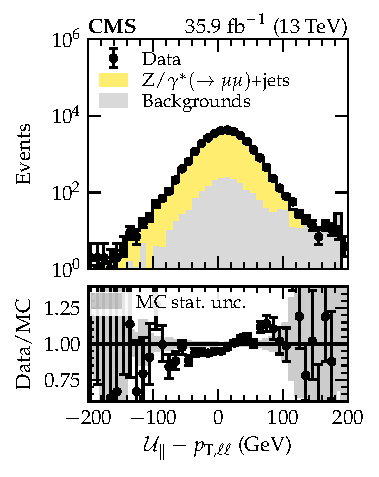
\includegraphics{chapters/041_corrections/images/ptmiss_calib/metres_para_mm_incdist.pdf}
        \caption{Dimuon parallel component}
        \label{subfiga:recoil-calib-dists}
    \end{subfigure}
    \hfill
    \begin{subfigure}[b]{0.49\textwidth}
        \centering
        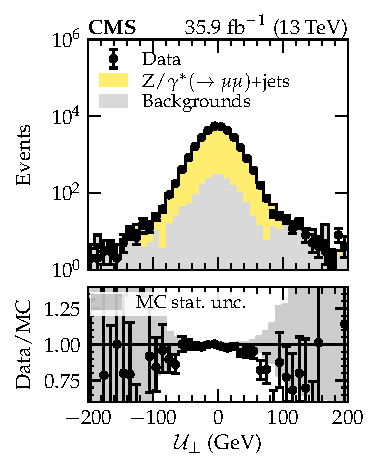
\includegraphics{chapters/041_corrections/images/ptmiss_calib/metres_perp_mm_incdist.pdf}
        \caption{Dimuon perpendicular component}
        \label{subfigb:recoil-calib-dists}
    \end{subfigure}
    \\
    \begin{subfigure}[b]{0.49\textwidth}
        \centering
        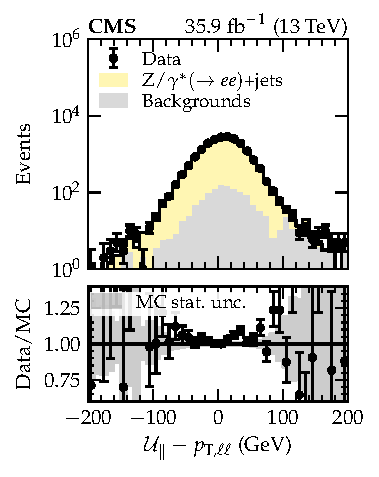
\includegraphics{chapters/041_corrections/images/ptmiss_calib/metres_para_ee_incdist.pdf}
        \caption{Dielectron parallel component}
        \label{subfigc:recoil-calib-dists}
    \end{subfigure}
    \hfill
    \begin{subfigure}[b]{0.49\textwidth}
        \centering
        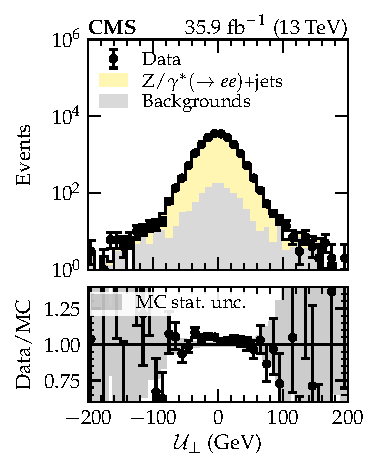
\includegraphics{chapters/041_corrections/images/ptmiss_calib/metres_perp_ee_incdist.pdf}
        \caption{Dielectron perpendicular component}
        \label{subfigd:recoil-calib-dists}
    \end{subfigure}
    \caption[Recoil distributions in dilepton final states.]{
        Distributions of the $\mathcal{U}_{\parallel}-\ptll$ and $\mathcal{U}_{\perp}$ for the \dimuplusjets and \dieleplusjets regions with the $\mathcal{U}$ requirement relaxed to ${\mathcal{U}>\SI{100}{GeV}}$ to probe their dependence with lower recoil while maintaining a reliable \ptmiss trigger scale factor measurement.
    }
    \label{fig:recoil-calib-dists}
\end{figure}

A maximum likelihood fit is performed to the data, with backgrounds subtracted by a template determined from MC, and the signal modelled as a Voigtian --- the convolution of a Gaussian with a Breit-Wigner which captures the peaking nature of the distribution smeared by the detector resolution. A large tail is seen in the backgrounds within the \recoilpara distribution as a result of processes with invisible particles leading to real \ptmiss, whereas the background in the \recoilperp distribution is symmetric. The Voigtian fit is also performed on the signal MC distribution to estimate the scale and resolution in MC. The scale is given by the mean of the distribution while the width is extracted as
%
\begin{equation}
    \sigma_V = \frac{1}{\sqrt{2\ln 2}}\left(0.5346\gamma + \sqrt{0.2166\gamma^2 + 2\ln(2) \sigma^2}\right)\ ,
\end{equation}
%
for a Voigtian with a Gaussian centred on $u_0$ and a width $\sigma$ and a Breit-Wigner also centred on $u_0$ and a width $\gamma$. When $\gamma\ll\sigma$ the distribution reduces to a Gaussian. These parameters are extracted from a fit in bins of \ptll since the detector resolution varies with the energy of particle tracks and deposits. The distribution of \ptll is shown in Fig.~\ref{fig:metres-zpt} which is divided into 20 bins of equal events in data, rounded to the nearest ${\SI{5}{GeV}}$ for convenience.
%
\begin{figure}[htb]
    \centering
    \begin{subfigure}[b]{0.49\textwidth}
        \centering
        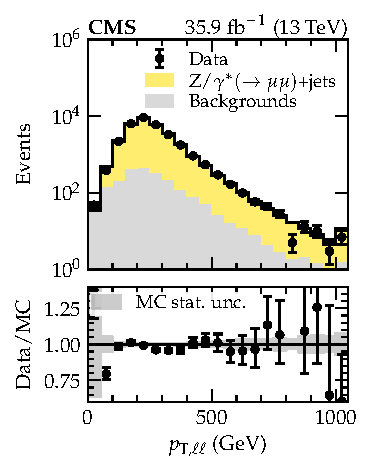
\includegraphics{chapters/041_corrections/images/ptmiss_calib/metres_ptll_mm_incdist.pdf}
        \caption{\dimuplusjets}
        \label{subfiga:metres-zpt}
    \end{subfigure}
    \begin{subfigure}[b]{0.49\textwidth}
        \centering
        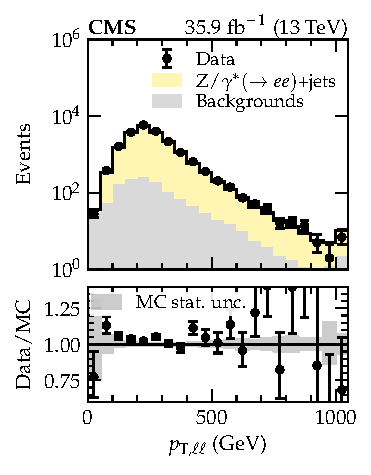
\includegraphics{chapters/041_corrections/images/ptmiss_calib/metres_ptll_ee_incdist.pdf}
        \caption{\dieleplusjets}
        \label{subfigb:metres-zpt}
    \end{subfigure}
    \caption[Dilepton \pt distribution.]{
        Dilepton \ptll distributions peaking near $\SI{200}{GeV}$ as a result of the kinematic selection placed on the recoil and the leading jet.
    }
    \label{fig:metres-zpt}
\end{figure}
%
The fit is performed in each \ptll bin with $\SI{10}{GeV}$ bins in the $\mathcal{U}_{\parallel}-\ptll$ and $\mathcal{U}_{\perp}$ dimensions. A prediction for the number of events in each bin is determined from the sum of the Voigtian and the MC background template. The signal normalisation is unconstrained and determined from the fit, along with the $u_0$, $\gamma$ and $\sigma_V$ parameters. Furthermore, the background contribution in each bin is constrained by a gamma distribution\footnote{The gamma distribution is the generalised poisson distribution to real numbers, such as for weighted events from simulations.} centred on the MC prediction. Occasionally the background contribution is negative as a result of NLO MC event generator weights leading to a negative probability density function in the maximum likelihood fit. To avoid the negative contributions, adjacent $\SI{10}{GeV}$ bins are merged until all background contributions are positive. This proves to be a robust method while maintaining a satisfactory number of bins. Additional fitting issues arise when the $\gamma$ parameter is near the lower limit at zero. In such cases the $\gamma$ parameter is fixed at zero and reliable results are recovered. These precautions are also used in the MC fits. Example fits in data and MC are shown in Fig.~\ref{fig:metres-fit-examples}. The good agreement in the data fit implies the statistical uncertainty in the background dominates over the systematic uncertainties. Conversely, the systematic uncertainties in the MC fit may dominate. To determine the effect of the systematic uncertainties, the MC fit is performed under the $\pm 1\sigma$ hypotheses for all systematic variations and the difference between the nominal fit parameters is taken as a systematic uncertainty. These are combined in quadrature for the final MC fit uncertainties. Most systematic uncertainties alter the normalisation of these distributions and hence do not impact the scale and the resolution. However, the lepton and jet energy scale uncertainties have the largest impact.

\begin{figure}[htb]
    \centering
    \begin{subfigure}[b]{0.49\textwidth}
        \centering
        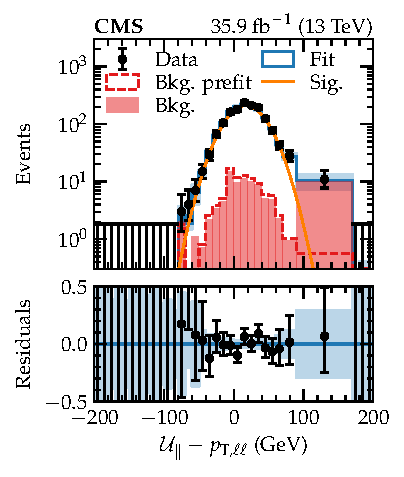
\includegraphics{chapters/041_corrections/images/ptmiss_calib/metres_datafit_example.pdf}
        \caption{Data fit}
        \label{subfiga:metres-fit-examples}
    \end{subfigure}
    \begin{subfigure}[b]{0.49\textwidth}
        \centering
        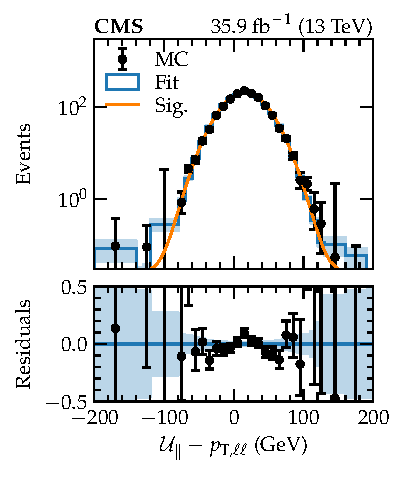
\includegraphics{chapters/041_corrections/images/ptmiss_calib/metres_mcfit_example.pdf}
        \caption{MC fit}
        \label{subfigb:metres-fit-examples}
    \end{subfigure}
    \caption[Fit result to extract the recoil scale and resolution in data and simulation.]{
        Fit results for the \ptll bin $180$--$\SI{190}{GeV}$ in data and MC; showing the fit result, background (Bkg.) prefit and postfit, signal Voigtian (Sig.) and the total fit result and it's uncertainty band; for the $\mathcal{U}_{\parallel}-\ptll$ distribution. The merging of bins is shown to remove negative probability density functions. The residuals represent the difference between the data points and the fit result with good agreement in the data fit and slightly worse in the MC fit as systematic uncertainties are not included to cover the discrepancy.
    }
    \label{fig:metres-fit-examples}
\end{figure}

The scale $u_0$ and resolution $\sigma_V$ extracted from the fits for each \ptll bin is shown in Fig.~\ref{fig:recoil-calib-ptllbins-mm} for the \dimuplusjets region and Fig.~\ref{fig:recoil-calib-ptllbins-ee} for the \dieleplusjets region.
%
\begin{figure}[htb]
    \centering
    \begin{subfigure}[b]{0.49\textwidth}
        \centering
        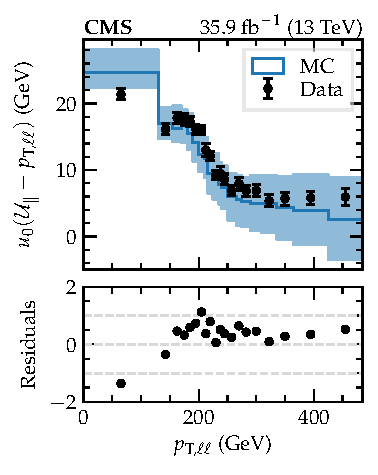
\includegraphics{chapters/041_corrections/images/ptmiss_calib/metres_mm_u0_para.pdf}
        \caption{Parallel scale}
        \label{subfiga:recoil-calib-ptllbins-mm}
    \end{subfigure}
    \hfill
    \begin{subfigure}[b]{0.49\textwidth}
        \centering
        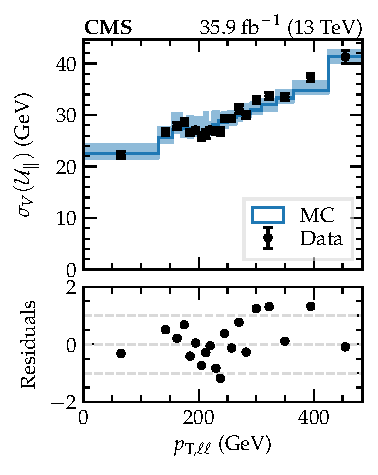
\includegraphics{chapters/041_corrections/images/ptmiss_calib/metres_mm_sigmav_para.pdf}
        \caption{Parallel resolution}
        \label{subfigb:recoil-calib-ptllbins-mm}
    \end{subfigure}
    \\
    \begin{subfigure}[b]{0.49\textwidth}
        \centering
        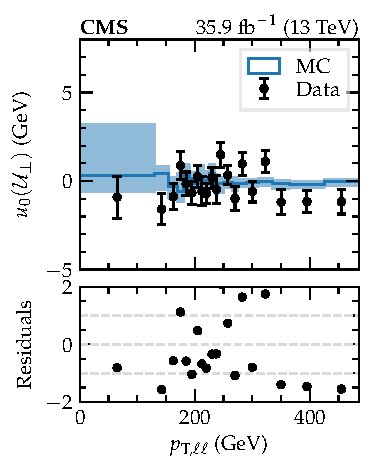
\includegraphics{chapters/041_corrections/images/ptmiss_calib/metres_mm_u0_perp.pdf}
        \caption{Perpendicular scale}
        \label{subfigc:recoil-calib-ptllbins-mm}
    \end{subfigure}
    \hfill
    \begin{subfigure}[b]{0.49\textwidth}
        \centering
        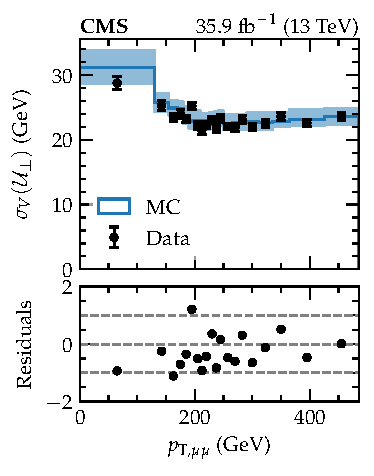
\includegraphics{chapters/041_corrections/images/ptmiss_calib/metres_mm_sigmav_perp.pdf}
        \caption{Perpendicular resolution}
        \label{subfigd:recoil-calib-ptllbins-mm}
    \end{subfigure}
    \caption[Recoil scale and resolution in the dimuon final state.]{
        The \ptmiss scale and resolution from the fit to data and MC in the \dimuplusjets region. The residuals represent the difference between data and MC, scaled by the reciprocal of the uncertainties added in quadrature.
    }
    \label{fig:recoil-calib-ptllbins-mm}
\end{figure}
%
\begin{figure}[htb]
    \centering
    \begin{subfigure}[b]{0.49\textwidth}
        \centering
        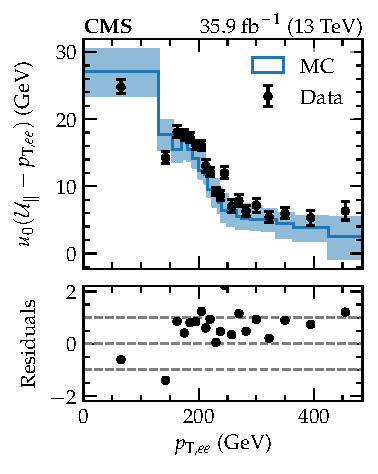
\includegraphics{chapters/041_corrections/images/ptmiss_calib/metres_ee_u0_para.pdf}
        \caption{Parallel scale}
        \label{subfiga:recoil-calib-ptllbins-ee}
    \end{subfigure}
    \hfill
    \begin{subfigure}[b]{0.49\textwidth}
        \centering
        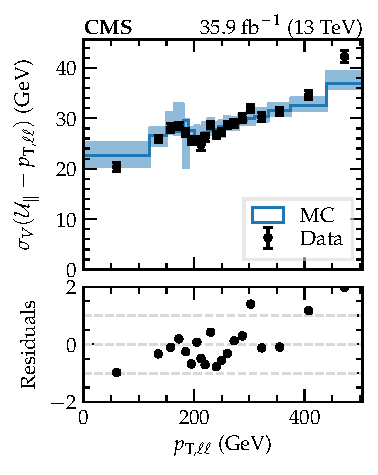
\includegraphics{chapters/041_corrections/images/ptmiss_calib/metres_ee_sigmav_para.pdf}
        \caption{Parallel resolution}
        \label{subfigb:recoil-calib-ptllbins-ee}
    \end{subfigure}
    \\
    \begin{subfigure}[b]{0.49\textwidth}
        \centering
        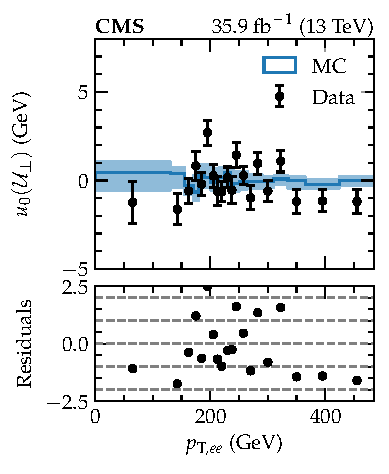
\includegraphics{chapters/041_corrections/images/ptmiss_calib/metres_ee_u0_perp.pdf}
        \caption{Perpendicular scale}
        \label{subfigc:recoil-calib-ptllbins-ee}
    \end{subfigure}
    \hfill
    \begin{subfigure}[b]{0.49\textwidth}
        \centering
        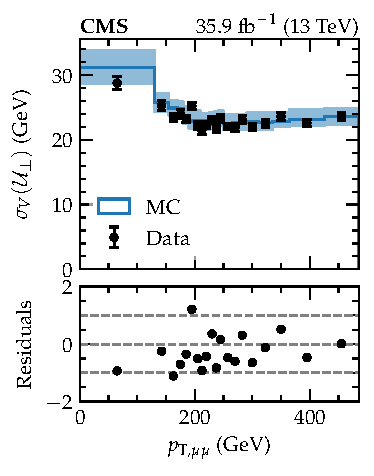
\includegraphics{chapters/041_corrections/images/ptmiss_calib/metres_ee_sigmav_perp.pdf}
        \caption{Perpendicular resolution}
        \label{subfigd:recoil-calib-ptllbins-ee}
    \end{subfigure}
    \caption[Recoil scale and resolution in the dielectron final state.]{
        Similar results to Fig.~\ref{fig:recoil-calib-ptllbins-mm} in the \dieleplusjets region.
    }
    \label{fig:recoil-calib-ptllbins-ee}
\end{figure}
%
The scale and resolution in both the \dimuplusjets and \dieleplusjets region agree within their respective uncertainties. Therefore, no additional corrections are derived for the scale or the resolution since the recoil as a proxy for the boson \pt is well-modelled in MC. A few outliers with residuals beyond $\pm 1$ are seen; however, the number is not significantly beyond expectations given the number of bins probed. Furthermore, the most important parameter, the parallel scale, shows an overestimate in the systematic uncertainties.

\clearpage
\section{Summary}

Corrections are applied to simulation to improve the modelling of data, typically determined from data-driven measurements of scale factors to correct the efficiency of a selection in MC to match the data efficiency, along with systematic uncertainties representing limitations in the scale factors.

The first set of corrections fix the emulated trigger efficiency in MC for the single muon and electron trigger paths measured in \IDYll events with the tag and probe method. The \ptmiss trigger scale factors are determined from events collected by the single muon trigger paths as a reference. Systematic uncertainties estimate the effect of the muon mismatch between the \SWT and offline selection, the use of the single muon trigger reference and variations from an independent region. After the trigger corrections are applied, object based selection corrections are measured, typically with the tag and probe method, for the muon identification and isolation; electron identification, isolation and reconstruction; photon identification and track veto; and jet $b$ and \Ptauh-tag identification.  Similarly, the energy and \pt scale corrections and systematic uncertainties are measured for muons, \Ptauh, electrons, photons and jets, all of which are propagated through the recoil calculation. Global event-based corrections and uncertainties are determined for the luminosity measurement, pileup reweighting, ECAL timing degradation and theory corrections to higher precision in QCD and electroweak vertices including QCD factorisation and renormalisation scale and PDF variations. The use of the recoil variable as a proxy for the boson \pt in \IZvvj, \IWlvj and \IDYllj processes is probed in \IDYllj events by splitting the recoil into a parallel and perpendicular component to extract the scale and resolution in both data and MC. The results show good agreement, within uncertainties, hence no additional corrections or systematic uncertainties are required.

All corrections are applied to the relevant processes in simulated events. Alternative distributions are provided under the $\pm 1\sigma$ variations for later likelihood fits to extract the \IZvvj and \IZllj event yields in determining the \PZ invisible width.
